\chapter{Introduction}

In this chapter, we first describe sequence tagging tasks and introduce the motivation of this thesis. Then, we summarize our major contributions and describe the structure of the thesis.

\section{Sequence Tagging Task}

\subsection{Part-of-Speech Tagging (POS)}
Part-of-Speech Tagging (POS) is a basic sequence tagging task, which assigns each word with a unique tag that indicates its syntactic role, such as noun, adverb, verb \dots Figure \ref{fig:pos-ex} illustrates a typical POS task. 

Most POS systems are evaluated on the English Penn TreeBank data set (\citeauthor{marcus1993building}, \citeyear{marcus1993building}), which contains 45 part-of-speech tags. The standard split uses section 1-18 of the Treebank for training, section 19-21 for tuning, and section 22-24 for testing (\citeauthor{toutanova2003feature}, \citeyear{toutanova2003feature}). The experimental data are summarized in Table \ref{table:my-dataset}. A lot of existing models are linear models, such as Maximum entropy Markov models (MEMMs) which obtains 96.46\% per word accuracy (\citeauthor{mccallum2000maximum}, \citeyear{mccallum2000maximum}); and the averaged perception discriminative model which obtains 97.11\% per word accuracy (\citeauthor{collins2002discriminative}, \citeyear{collins2002discriminative}). More recently, neural network models are proposed to improve the state-of-the-art score. The Bidirectional LSTM network model proposed by \cite{huang2015bidirectional} reaches 97.55\% per word accuracy. \cite{ling2015finding} presents the compositional character-to-word LSTM model which reaches the state-of-the-art performance: 97.78\% per word accuracy. The performance of existing POS models is reported in Table \ref{table:my-performance}.

\begin{table}[]
\centering
\caption{Number of Sentences (words) and Labels in Each Training, Validation and Test Section of Different Data Sets}
\label{table:my-dataset}
\begin{tabular}{|c|c|c|c|c|} \hline
      & Training  & Validation  & Test  & labels  \\ \hline
Penn Treebank   &39831(950011) &1699(40068) &2415(56671) &45\\\hline
CoNLL2003   &14987(204567) &3466(51578) &3684(46666) &9     \\\hline
OntoNotes   &75187(1088503) &9479(147724) &9603(152728) &18     \\\hline
\end{tabular}
\end{table}


\begin{table}[]
\centering
\caption{Performance of Different POS and NER Systems}
\label{table:my-performance}
\begin{tabular}{cclcc}
POS Systems       & Accuracy &  & NER Systems           & F1
\\ \cline{1-2} \cline{4-5} 
\text{\cite{mccallum2000maximum}} & 96.46\%                      &  & \text{\cite{florian2003named}}                 & 88.76                  \\
\text{\cite{collins2002discriminative}}    & 97.11\%                      &  & \text{\cite{huang2015bidirectional}}           & 88.83                  \\
\text{\cite{huang2015bidirectional}}       & 97.55\%                      &  & \text{\cite{lample2016neural}} with CRF        & \textbf{90.94}                 \\
\text{\cite{ling2015finding}}              & \textbf{97.78}\%                      &  & \text{\cite{lample2016neural}} with Stack LSTM & 90.33                 
\end{tabular}
\end{table}



\subsection{Named Entity Recognition (NER)}

Named Entity Recognition (NER) is a more complex sequence tagging task than POS, which identifies expressions
that refer to named entities, such as peoples, places, organizations and others. The main difference between NER and POS is that each named entity label can span multiple words while each part-of-speech tag is only for one word. A popular convention in NER is to use the "IOB" label scheme (Inside, Outside, Beginning): if the word is the beginning of a named entity label, it is marked as B-label; if the word is inside a named entity tag but not the first one, it is marked as I-label; if the token is outside the named entity, it is labeled as O. An example of NER is shown in Figure \ref{fig:ner-ex}. There are different number of named entity types in different NER tasks. For example, the shared task of CoNLL 2003 (~\citeauthor{tjong2003introduction}, ~\citeyear{tjong2003introduction}) contains 4 types of named entities: locations (LOC), persons (PER), organizations (ORG), and miscellaneous (MISC); and the OntoNotes English data set (~\citeauthor{hovy2006ontonotes}, ~\citeyear{hovy2006ontonotes}) contains 18 types of named entities shown in Table \ref{table:ontonotes-type}. The predefined training, development, and testing split of the data sets are shown in Table ~\ref{table:my-dataset}.

\begin{table}[]
\centering
\caption{Name Entity Types in OntoNotes}
\label{table:ontonotes-type}
\begin{tabular}{|c|c|} \hline
Types  & Named Entities  \\ \hline
PERSON & People, including fictional \\ \hline
NORP & Nationalities or religious or political groups \\\hline
FACILITY & Buildings, airports, highways, bridges, etc. \\ \hline
ORG & Companies, agencies, institutions \\ \hline
GPE & Countries, cities, states \\ \hline
LOC & Non-GPE locations, mountain ranges, bodies of water \\ \hline
PRODUCT & Vehicles, weapons, foods, etc. (Not services) \\ \hline
EVENT & Named hurricanes, battles, wars, sports events \\ \hline
WORK OF ART & Titles of books, songs \\ \hline
LAW & Named documents made into laws \\ \hline
LANGUAGE & Any named language  \\ \hline
DATE & Absolute or relative dates or period \\ \hline
TIME & Times smaller than a day  \\ \hline 
PERCENT & Percentage \\ \hline
MONEY & Monetary values, including unit \\ \hline
QUANTITY & Measurements, as of weight or distance \\ \hline
ORDINAL & first, second, etc. \\ \hline
CARDINAL & Numerals that do not fall under another type \\ \hline
\end{tabular}
\end{table}

Most NER models are evaluated on CoNLL 2003 data set and are measured by the F1 score, which is the harmonic mean of precision and recall. 

\begin{equation}\label{eqn:softmax}
F_{1} = 2\times \dfrac{\textit{precision} \times \textit{recall}}{\textit{precision} + \textit{recall}}
\end{equation}

Since CoNLL 2003 has a relatively smaller size of training data, most of the existing models make use of pretrained word embeddings along with the training data. A commonly used pretrained word embeddings is GloVe (\citeauthor{pennington2014glove}, \citeyear{pennington2014glove}) which contains 40K words. The best system presented at the NER CoNLL 2003 challenge by \cite{florian2003named} obtains 88.76 F1 score. The model using Bidirectional LSTM by \cite{huang2015bidirectional} reaches 88.83 F1 score. Both of these two models use a lot of external features along with gazetteer\footnote{Gazetteers are language-specific knowledge resources}. \cite{lample2016neural} proposed two NER models with no external features or a gazetteer: the first one makes structured prediction uses Bidirectional LSTM, Character Embeddings (\citeauthor{ling2015finding}, \citeyear{ling2015finding}) and Conditional Random Field (CRF) (\citeauthor{lafferty2001conditional}, \citeyear{lafferty2001conditional}); and the second one uses a Shift-Reduce framework with Stack-LSTM (\citeauthor{dyer2015transition}, \citeyear{dyer2015transition}). The first model achieves the state-of-the-art F1 score, while the second one performs slightly worse. The performance of existing NER models is reported in Table \ref{table:my-performance}.


%\textbf{GLoVE} It's been shown that using pretrained word embeddings leads to significant performance improvement on sequence tagging (~\citeauthor{collobert2011natural}, ~\citeyear{collobert2011natural}; ~\citeauthor{lample2016neural}, ~\citeyear{lample2016neural}).


\begin{figure}
  \centering
  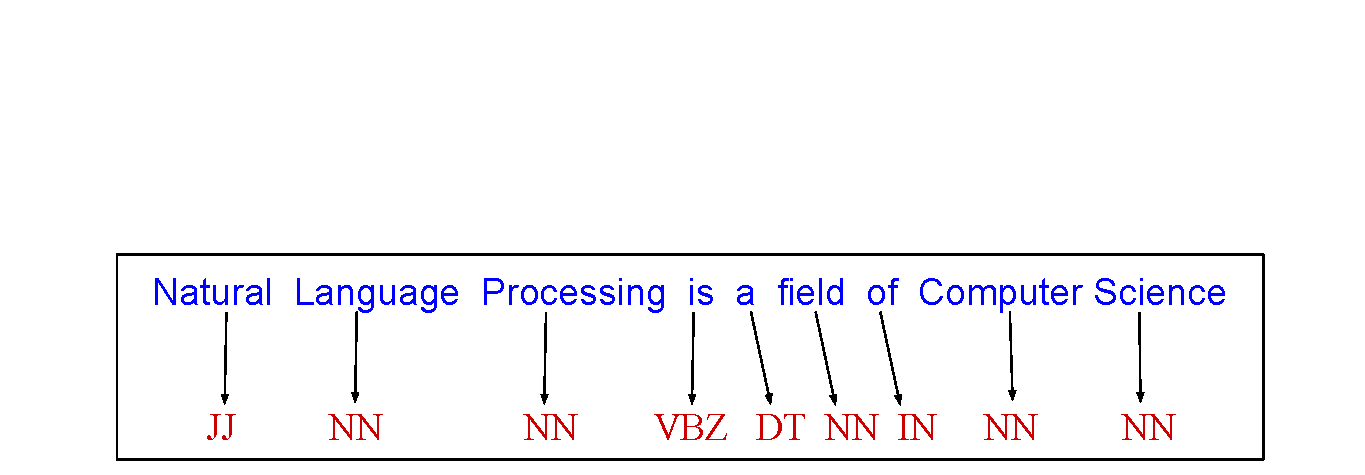
\includegraphics[scale=0.5]{posex.pdf}
 \caption{An example of POS}
  \label{fig:pos-ex}
\end{figure}

\begin{figure}
  \centering
  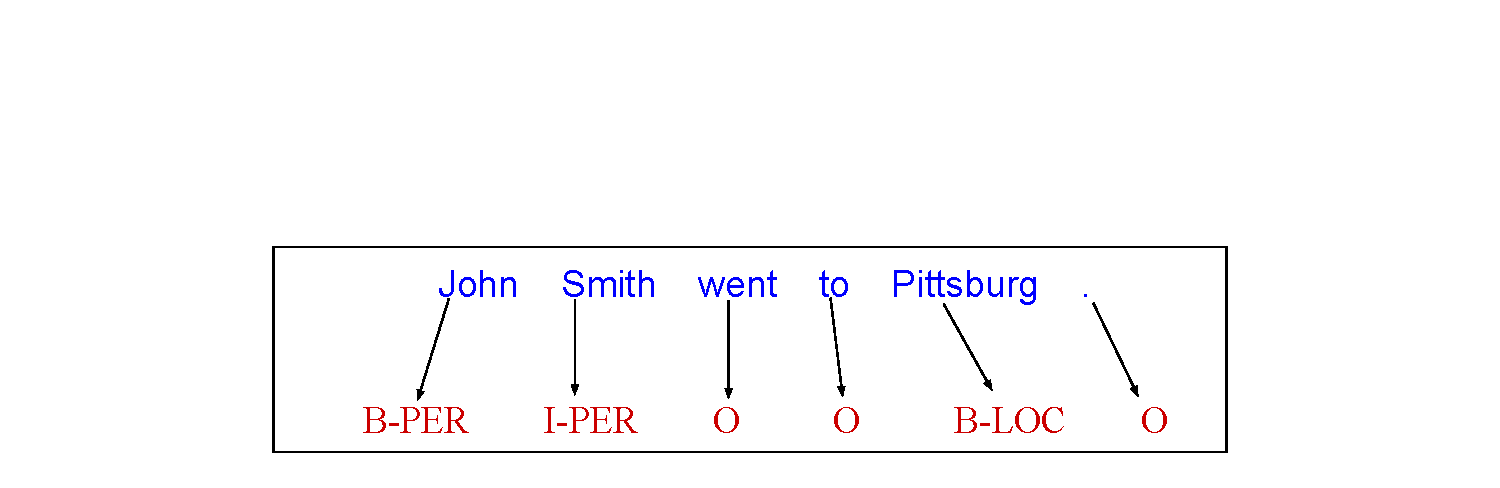
\includegraphics[scale=0.5]{nerex.pdf}
 \caption{An example of NER}
  \label{fig:ner-ex}
\end{figure}

\section{Motivation}
Recurrent Neural Networks (RNNs) have obtained impressive results in many NLP tasks, such as speech recognition (\citeauthor{graves2013speech}, \citeyear{graves2013speech}) and machine translation (\citeauthor{cho2014properties}, \citeyear{cho2014properties}).
Bidirectional Long Short Term Memory (BiLSTM) (\citeauthor{Hochreiter97longshort-term}, \citeyear{Hochreiter97longshort-term}; \citeauthor{graves2005framewise}, \citeyear{graves2005framewise}) is one of the RNN architectures that can maintain long-distance information from the past and future data in a input sequence. Based on the existing work (POS system by \cite{ling2015finding} and NER system by \cite{lample2016neural}), state-of-the-art results on POS and NER can be obtained by using a BiLSTM network with Character Embeddings and CRF. Some work has also shown that feedforward neural networks can achieve comparable accuracy with recurrent models in tasks such as POS and Dependency Parsing (\citeauthor{andor2016globally}, \citeyear{andor2016globally}). One approach presented in this thesis is to employ a greedy transition system with a feedforward network to make independent classification decision on each word. However, the greedy system is limiting when there are strong correlations between output labels. NER is one of such tasks which have grammar constrains on output label sequences. For example, "I-PER" cannot follow "B-LOC" in NER. In order to take into account the strong dependencies among output labels, a CRF layer is added to model the output label sequence jointly. Since the CRF-based models focus on the sentence level and compute the score of every possible sequence, they take more time in training and decoding. Since we are interested in the decoding speed and performance trade-off in different neural network models, we re-implement variants of feedforward models and BiLSTM models using Tensorflow (\citeauthor{abadi2016tensorflow}, \citeyear{abadi2016tensorflow}) and systematically compare the performance and decoding speed between them on sequence tagging tasks, such as POS and NER.

Since the named entity labels in NER often span multiple tokens, most neural architectures for NER predict the boundaries and types of entities together using the the "IOB" label scheme. Mention2Vec (\citeauthor{stratos2016mention2vec}, \citeyear{stratos2016mention2vec}) is proposed to address the natural segment-level representation in NER by separating the NER task into boundary detection (I, O, B) and type prediction (PER, LOC, etc.). While Mention2Vec employs two BiLSTMs for each sub-task, we replace the BiLSTM layer for boundary detection with a feedforward network in order to obtain a simpler model and accelerate the decoding process. This new model is denoted as Feedforward-Mention2Vec in this thesis.

We use Byte Pair Encoding (BPE) (\citeauthor{gage1994new}, \citeyear{gage1994new}) to deal with rare words in sentences for machine translation(\citeauthor{sennrich2015neural}, \citeyear{sennrich2015neural}), and we propose a new model combining BPE and Mention2Vec for POS, which is denoted as BPE-Mention2Vec in this thesis. We use BPE to segment the input words in the hope of capturing the orthographic evidence of the words without using spelling features (like prefixes and suffixes) or Character Embeddings. After we segment input words, POS becomes a NER-like task. Then, we can use Mention2Vec to solve the rest of the problem. Since boundaries of output tags are known in POS, we only need to use a BiLSTM network for type prediction in \mb.

\section{Contribution}
The three main contributions of this thesis are:

\begin{enumerate}

\item We implement two greedy tagging systems with two different feedforward network models, \ffa{} and \ffb. 

\ffa{} takes word features in context, spelling features, and history tag features as input. \ffb model uses word features in context and CRF to model the output sequences jointly. There are few work measuring the decoding time using feedforward networks on sequence tagging, so We conduct the experiments on NER and POS and record the performance and decoding speed on Penn Treebank data for POS and CoNLL 2003 data for NER. To test the robustness of the feedforward networks, we also conduct experiments using a feedforward network with only word features, which also serves as the baseline. We compare different feedforward models and provide analysis on the results. 

\item In addition to the greedy tagging systems with different feedforward networks, we build a tagging system using the fully structured BiLSTM model, which makes use of Character Embeddings and CRF. 

There is few work examining how the configurations of the fully structured BiLSTM model affect the decoding speed, such as if the model is using Character Embeddings or if the model is using CRF. We conduct experiments to compare the performance and decoding time of different configurations on POS and NER. We also benchmark the BiLSTM models against the feedforward models.

\item Last but not least, we introduce two new neural architectures based on Mention2Vec: Feedforward-Mention2Vec for NER and BPE-Mention2Vec for POS. 

Originally, Mention2Vec is designed for NER which uses BiLSTMs to detect named entity boundaries and predict corresponding types separately. We propose Feedforward-Mention2Vec for NER, in which we use a feedforward network with CRF to predict named entity boundaries instead of using a BiLSTM.  We denote this new model for NER as \ma. We also adapt Mention2Vec for POS by combining Byte Pair Encoding (BPE) with BiLSTM in the model. BPE is used to segment the input words in our model, and it converts POS into a NER-like task. We denote this new model for POS as \mb. In BPE-Mention2Vec, we use a feedforward network to compute the hidden embeddings of the input segmented words. Since the boundaries of subword units are known, \mb{} does not need to predict the boundaries. It takes the hidden embeddings, tag boundaries, and a BiLSTM network to predict the actual POS tags. We benchmark these two multi-task models against the state-of-the-art BiLSTM model on POS and NER. Since different NER tasks have different number of named entity types, the decoding time of fully structured BiLSTM model grows quadratically in the number of types. In Mention2Vec and Feedforward-Mention2Vec, we only apply CRF on boundary labels (I, O, B), so the decoding time grows linearly in the number of types. To show the time difference on different NER tasks, we conduct the NER experiments on CoNLL 2003 which contains 4 different named entity types and OntoNotes which contains 18 different named entity types.

\end{enumerate}


\section{Overview}
The thesis is organized as follows:

In \textbf{Chapter 2}  we present three different feedforward network models: feedforward network with only word features (denoted as Feedforward); feedforward network with spelling features and history features (denoted as \ffa); and feedforward network with CRF (denoted as \ffb). We explain the training and decoding process of the feedforward models, demonstrate the experiment design, and compare the performance and decoding time between different feedforward models.

In \textbf{Chapter 3} we present the fully structured BiLSTM model (a combination of BiLSTM, Character Embeddings and CRF), denoted as the BiLSTM-Char-CRF model. We explain the training and decoding process of BiLSTM-Char-CRF, and conduct experiments using three different configurations: BiLSTM with word features only, BiLSTM with Character Embeddings, and BiLSTM model with Character Embeddings and CRF.

In \textbf{Chapter 4} we present two new new multi-task models based on Mention2Vec: Feedforward-Mention2Vec for NER and BPE-Mention2Vec for POS. We explain the architectures of these two models and we compare the performance and speed between multi-task models and BiLSTM models.

In \textbf{Chapter 5} we discuss the empirical results from the previous chapters. We also analyze the trade-off between performance and speed in different neural network models.

In \textbf{Chapter 6} we summarize the contributions of this thesis and discuss the ongoing and related future work.